\chapter{Obtención de geometría}

La reconstrucción tridimensional de una superficie es la construcción de un modelo que la representa, se define una correspondencia entre los puntos del modelo y de la superficie real. En esta sección se presentan distintas técnicas y métodos que permiten la construcción de modelos, discutiendo distintas características según propiedades de la superficie a representar y de la tecnología utilizada. Un conjunto de puntos, también llamado nube de puntos  es la representación de una superficie utilizada por varias técnicas y dispositivos. Utilizando procesamientos de datos se puede obtener información adicional entre los puntos, como normales que identifiquen orientación de la superficie, y subgrupos de puntos que representan caras de una malla. La construcción del modelo se presenta en dos etapas, inicialmente obteniendo puntos de la superficie y luego procesando los datos para completar el modelo.

\section{Correspondencia}

\subsection{Calibración}

Al calcular coordenadas tridimensionales a partir de imágenes obtenidas por capturas de video se introducen errores propios del modelo (modelo pinhole, modelo imaginario que utiliza una cámara) por ello es necesario hacer una corrección obteniendo una correspondencia entre el modelo real y el ideal, la calibración puede utilizarse como método para obtener la correspondencia mencionada. Luego de la calibración las coordenadas obtenidas son en dos dimensiones, corresponden a la proyección sobre el plano imagen, para completar las coordenadas tridimensionales en el modelo es necesario calcular la profundidad de cada punto, con este fin se utiliza el método de triangulación. El modelo ideal que se utiliza en las cámaras es el modelo pinhole, éste se presenta para un caso básico, se considera que el centro de proyección $C$ coincide con el origen del sistema de coordenadas, y que $Z = f$ (plano imagen o plano focal).

\begin{figure}[H]
  \centering
    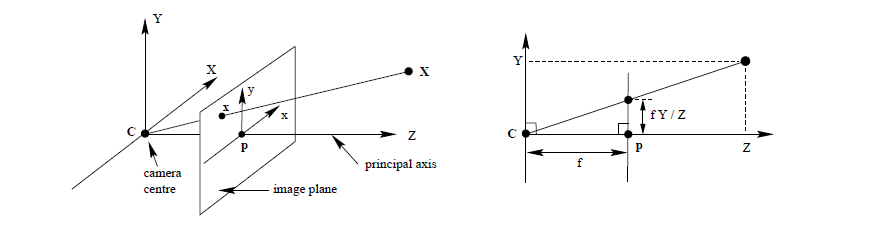
\includegraphics[width=0.5\textwidth]{./Cap6_reconstruccion/pinhole.png}
  \caption{Geometría de cámara pinhole. $C$ es centro de la cámara y $p$ el punto principal}
  \label{fig:Calib-Pinhole}
\end{figure}

Un punto en el espacio $X=(X,Y,Z)^T$ se corresponde con el punto $X$ en el plano imagen, dado por la intersección del rayo que pasa por el centro de cámara y el punto $X$ con el plano imagen, el punto $(X,Y,Z)^T$ es mapeado con $(\frac{f_X}{Z}, \frac{f_Y}{Z}, f)^T$ en el plano imagen.
$(X, Y, Z)^T \to (\frac{f_X}{Z}, \frac{f_Y}{Z},f)^T$ se considera que el centro de coordenadas del plano imagen coincide con el punto principal $P$.
El centro de proyección $C$ es el centro de la cámara o centro óptico.
Proyección central utilizando coordenadas homogéneas:
Considerando la representación de los puntos como vectores homogéneos se expresa la proyección central como una correspondencia lineal entre las coordenadas homogéneas:

\[
\begin{pmatrix}
X \\ Y \\ Z \\ 1
\end{pmatrix}
\to
\begin{pmatrix}
f_X \\ f_Y \\ Z
\end{pmatrix}
=
\begin{pmatrix}
f & 0 & 0 & 0 \\
0 & f & 0 & 0 \\
0 & 0 & 1 & 0 \\
\end{pmatrix}
\begin{pmatrix}
X \\ Y \\ Z \\ 1
\end{pmatrix}
\]

Dados $X = (X,Y,Z,1)^T$ y $x =(x,y,z)^T$ la correspondencia utilizando el método pinhole es:
$x=PX$

Siendo
\[
P = 
\begin{pmatrix}
f & 0 & 0 & 0 \\
0 & f & 0 & 0 \\
0 & 0 & 1 & 0 \\
\end{pmatrix}
\]

Considerando el caso general en el cual el centro de coordenadas del plano de proyección no coincide con el punto principal $P$ (las coordenadas de $P$ son $(p_x,p_y)^T$ ) la correspondencia es dada según:
$(X,Y,Z)^T \to (\frac{fX}{Z} + p_x, \frac{fY}{Z} + p_y, f)^T$

\[
\begin{pmatrix}
X \\ Y \\ Z \\ 1
\end{pmatrix}
\to
\begin{pmatrix}
f_X + Z * p_x \\ f_Y + Z * p_y \\ Z
\end{pmatrix}
=
\begin{pmatrix}
f & 0 & p_x & 0 \\
0 & f & p_y & 0 \\
0 & 0 & 1 & 0 \\
\end{pmatrix}
\begin{pmatrix}
X \\ Y \\ Z \\ 1
\end{pmatrix}
\]

\[
K =
\begin{pmatrix}
f &   & p_x & \\
  & f & p_y & \\
  &   & 1   & \\
\end{pmatrix}
\]

$K$ es la matriz de calibración, y se utilizará para obtener la correspondencia de cada punto según:
$x = K [I|0] X$
(siendo $[I|0]$ la matriz identidad sumado a una columna de ceros)
$X = (X,Y,Z,1)^T$ coordenadas espaciales considerando que el centro de la cámara coincide con el origen de coordenadas del sistema Euclidiano.
$x = (x, y, z)$ coordenadas que se buscan determinar.
En caso de considerar que el centro de coordenadas de la cámara no coincide con el origen de coordenadas del sistema Euclidiano es necesario utilizar una traslación y rotación para lograr esta correspondencia[1].%%%REFERENCIAR%%%

\subsection{Método de triangulación}
Este método determina las coordenadas $(x,y,z)$ de un punto utilizando la posición del punto obtenida en las perspectivas de dos proyecciones dadas.
Los centros de perspectiva y planos de proyección son conocidos [3].%%%REFERENCIAR%%%
Escena con dos dimensiones (2D)

\begin{figure}[H]
  \centering
    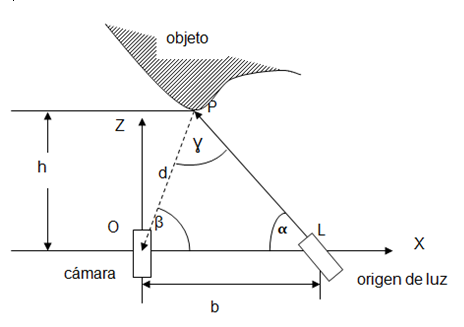
\includegraphics[width=0.5\textwidth]{./Cap6_reconstruccion/triangulacion.PNG}
  \caption{}
  \label{fig:Triangulacion}
\end{figure}

Este método tiene como objetivo calcular la distancia $d$ de la cámara al punto $P$ a partir de los datos: ángulos $\hat\alpha$, $\hat\beta$ y la distancia $b$ entre el proyector y la cámara.
El ángulo $\hat\alpha$ y la distancia $b$ son dados por la calibración de la escena.
El ángulo $\hat\beta$ esta dado por la geometría de la proyección.

\[
\left.
\begin{array}{l}
\frac{d}{\sin (\hat\alpha)} = \frac{b}{\sin (\hat\gamma)} 	\\
\gamma = \pi - (\alpha + \beta)								\\
\sin (\pi - \gamma) = \sin (\gamma)
\end{array}
\right \rbrace
\frac{d}{\sin(\gamma)} = \frac{b}{\sin(p - \gamma)} = \frac{b}{\sin(\alpha + \beta)} \Rightarrow d = b . \frac{\sin(a)}{\sin(\alpha + \beta)}
\]